%%%%%%%%%%%%
%%%%%%%%%%%%%%%%%%%%%%%%%%%%%%%%%%%%%%%%%%%
\begin{frame}{UDC}{Block diagram}
	\begin{figure}
		\centering
		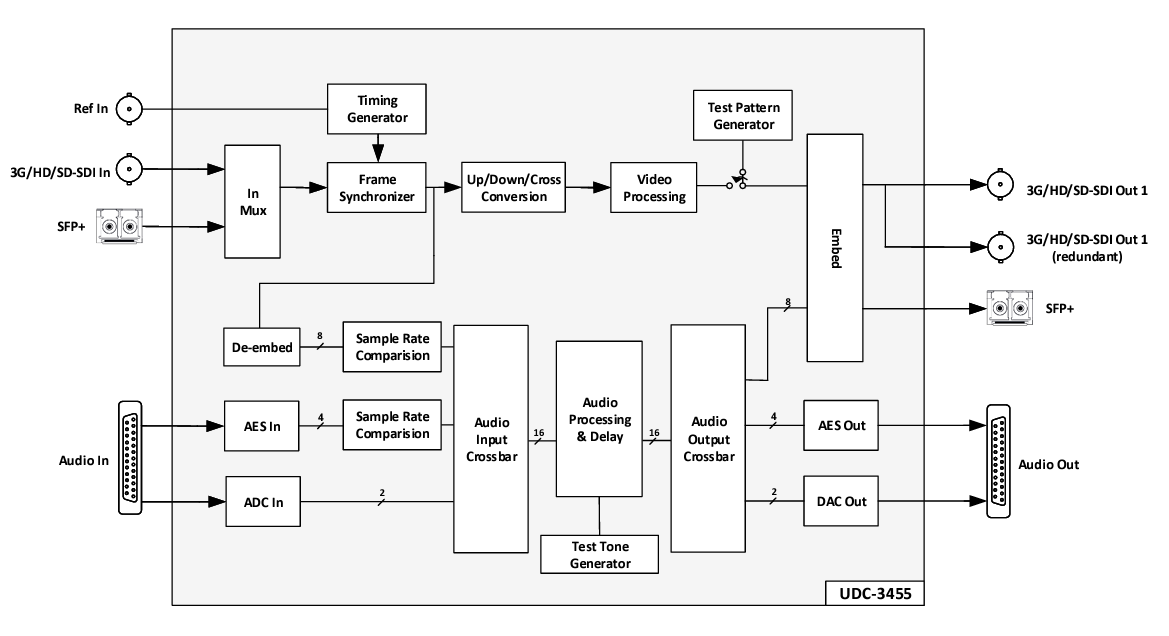
\includegraphics[scale=1]{graphics/block_diagram.png}
		\caption{UDC Block diagram}
	\end{figure}
\end{frame}
%%%%%%%%%%%%%%%%%%%%%%%%%%%%%%%%%%%%%%%%%%%
\begin{frame}{Audio syncronization}{ASRC}
	\begin{figure}
		\centering
		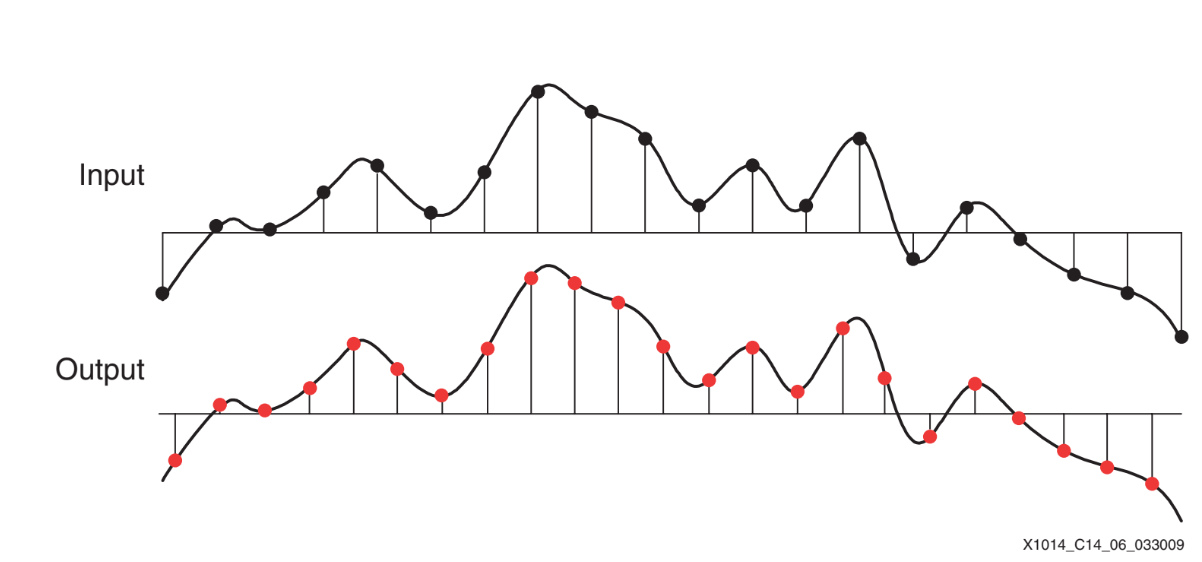
\includegraphics[scale=1]{graphics/asrc1.png}
		\caption{Sample Rate Conversion}
	\end{figure}
\end{frame}
%%%%%%%%%%%%%%%%%%%%%%%%%%%%%%%%%%%%%%%%%%%
\begin{frame}{Audio syncronization}{ASRC}
	\begin{figure}
		\centering
		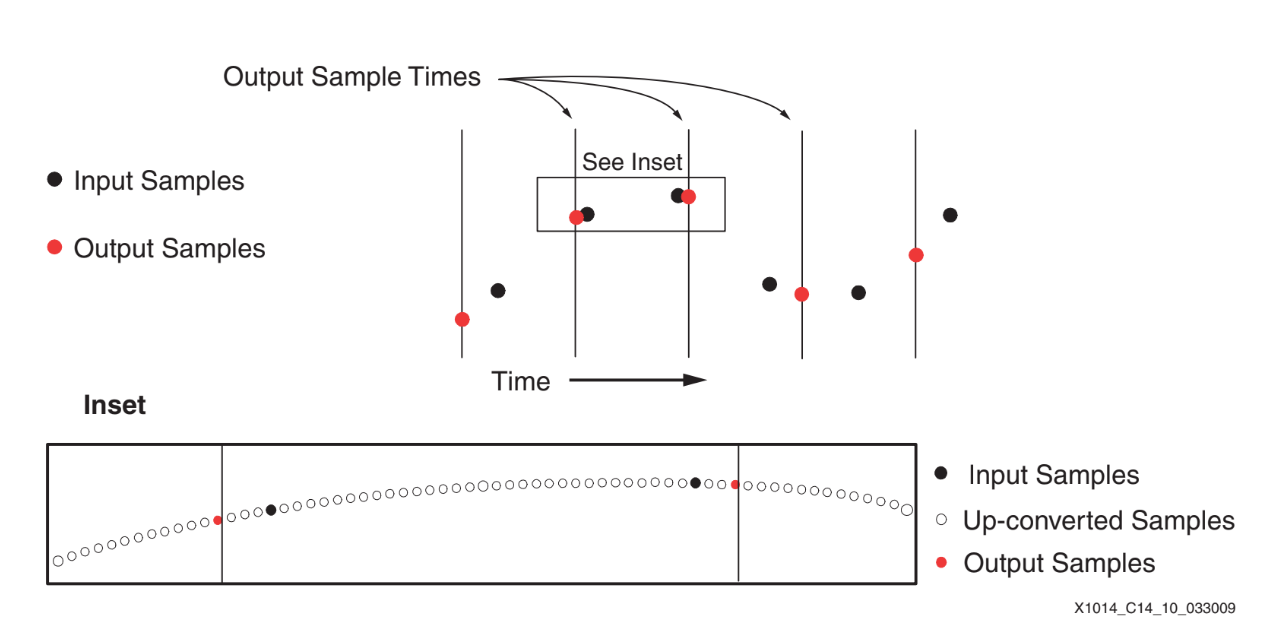
\includegraphics[scale=1]{graphics/asrc2.png}
		\caption{Classic Method of Asynchronous Sample Rate Conversion}
	\end{figure}
\end{frame}
%%%%%%%%%%%%%%%%%%%%%%%%%%%%%%%%%%%%%%%%%%% 
\begin{frame}{Video syncronization}{VDMA framesync}
	\begin{block}{Spectrum analyzer type:}
		\begin{itemize}
			\item Swept-tuned spectrum analyzer
			\item Vector signal analyzers
			\item Real-time spectrum analyzers (RTSA)
		\end{itemize}
	\end{block}
	\pause
	\begin{block}{}
		Real-time spectrum analysis allows a spectrum analyzer to conduct continuous,
		gapless capture and analysis of elusive and transient signals, while conventional
		spectrum analyzers and vector signal analyzers do not have this capability due to their design.
	\end{block}
\end{frame}
%%%%%%%%%%%%%%%%%%%%%%%%%%%%%%%%%%%%%%%%%%%